\documentclass[a4paper,12pt]{article}

% Deixar paginas Black 
%\usepackage{xcolor}
%\\pagecolor{black}
%\\color{white}

\usepackage[
  paperwidth=25.0cm,
  paperheight=200.0cm,
  left=1cm,
  right=1cm,
  top=0cm,
  bottom=0cm
]{geometry}

\usepackage{graphicx}  % No preâmbulo
\emergencystretch=3em
\hbadness=10000  % Ignora completamente underfull boxes
\tolerance=9999
% Pacotes básicos
%\usepackage[utf8]{inputenc}
\usepackage[T1]{fontenc}
\usepackage[brazil]{babel}
\usepackage{amsmath, amssymb}
\usepackage{hyperref}
\usepackage{xcolor}   % Necessário para cores

\title{\centering C Como Programar - pag. 472}

\author{}
\date{}

\begin{document}
\maketitle{}

{\centering 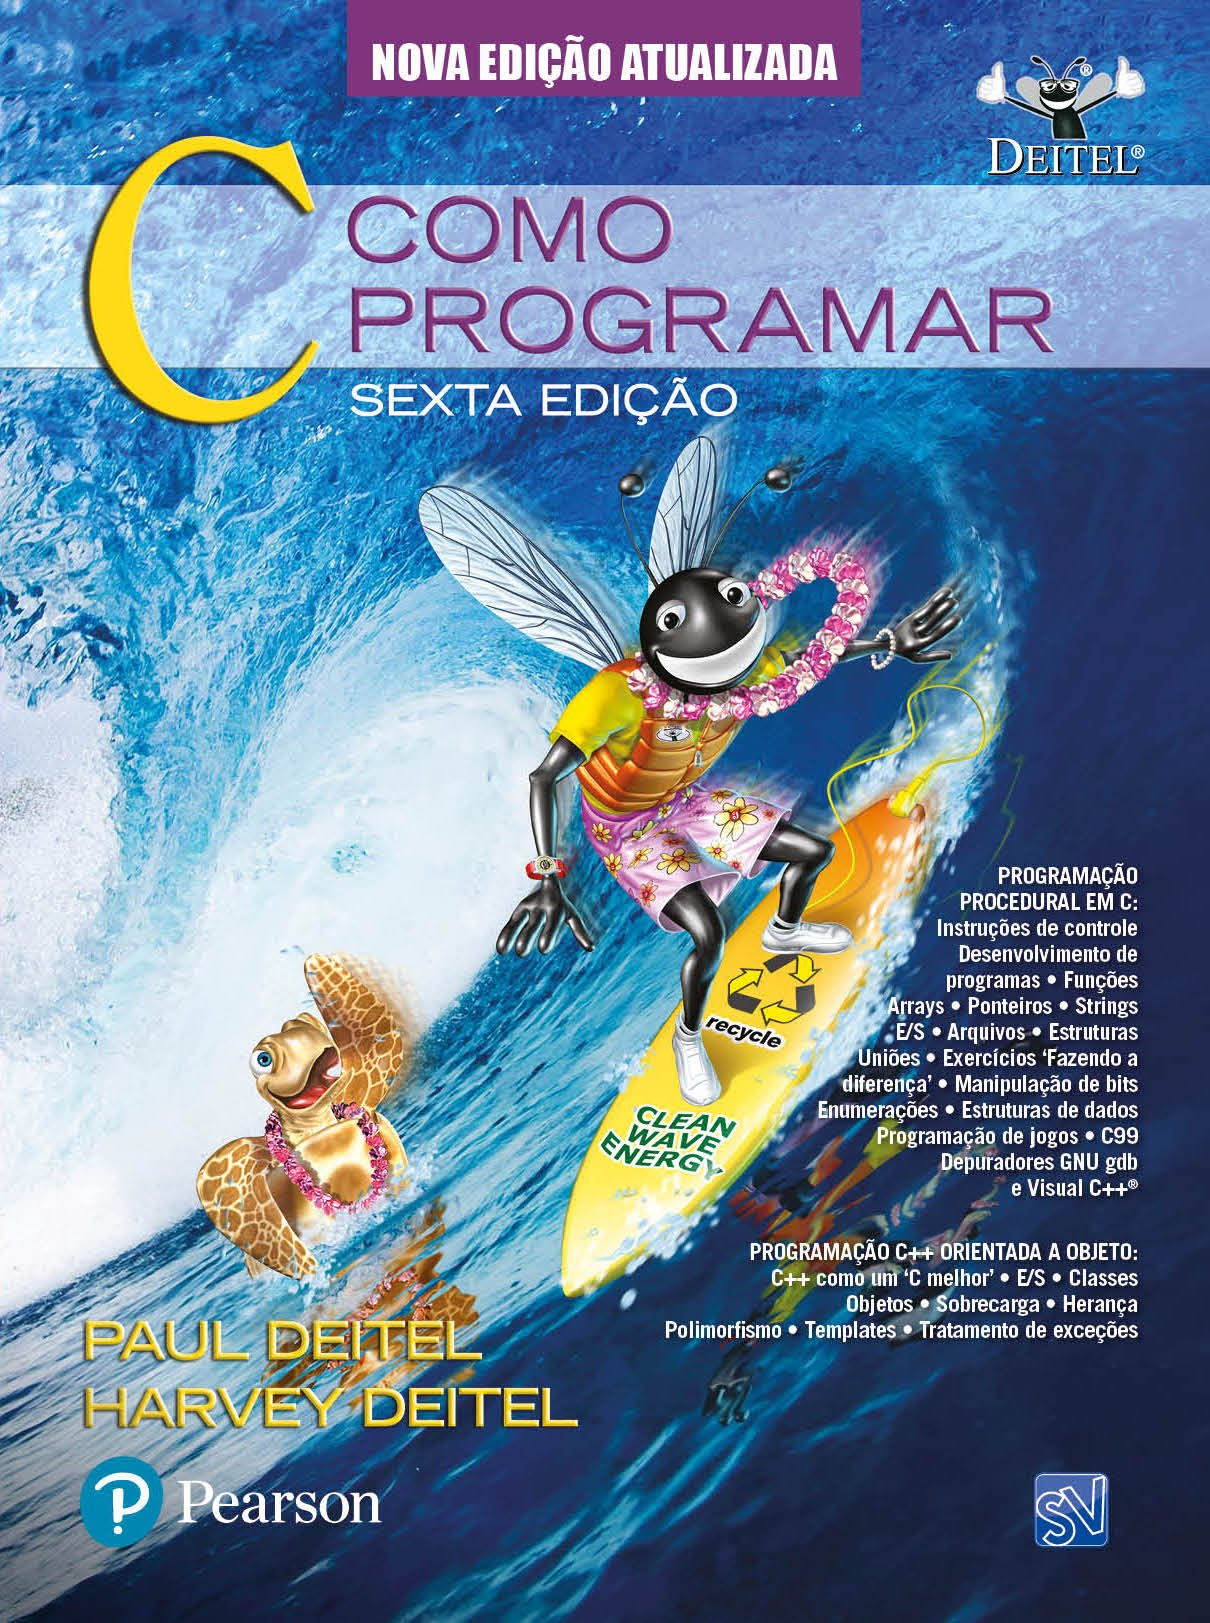
\includegraphics[width=5cm]{res/ebook.jpg} \par}


\section*{Frase marcante}
Conhecer algo nao é so saber como fuciona e sim entender todas as razoes de sua existencia, 
\section*{comessa aqui}


\section*{Exercicios}
\subsection*{2.1}
a) \texttt{main}    \\
b) \texttt{\{\}}    \\
c) \texttt{;}       \\
d) \texttt{stdio.h} \\
e) \texttt{NewLine} \\
f) \texttt{scanf()} \\
g) \texttt{\%}      \\
h)  \\
i)  \\
j) \texttt{if, elseif, else}

\subsection*{2.2}
a) \texttt{False}  \\
b) \texttt{False}  \\
c) \texttt{true}   \\
d) \texttt{true}   \\
e) \texttt{true}   \\
f) \texttt{False}  \\
g) \texttt{true}   \\
h) \texttt{true}   \\
i) \texttt{true}   \\
j) \texttt{False}  \\
k) \texttt{False}  \\
l) \texttt{False}  \\        

\subsection*{2.3}
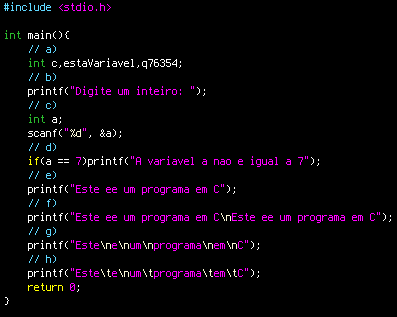
\includegraphics[width=0.3\textwidth]{res/image1.png}
\subsection*{2.4}
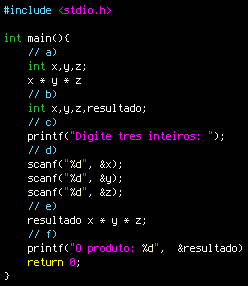
\includegraphics[width=0.3\textwidth]{res/image3.png}
\subsection*{2.5}
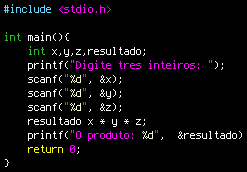
\includegraphics[width=0.3\textwidth]{res/image4.png}
\subsection*{2.6}
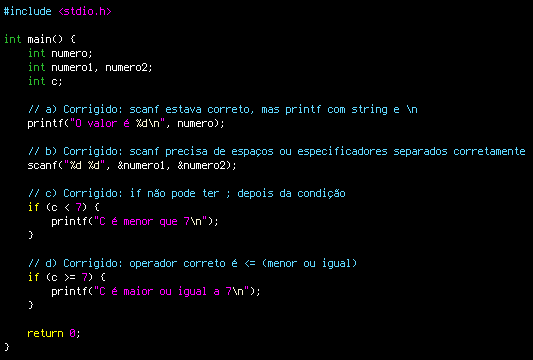
\includegraphics[width=0.3\textwidth]{res/image5.png}
\subsection*{2.7}
\begin{enumerate}
    \item[a)] \texttt{scanf("\%d", \&valor);}

    \item[b)] \texttt{printf("O produto de \%d e \%d e \%d\textbackslash n", x, y, z);}

    \item[c)] \texttt{x + y == z}

    \item[d)] \texttt{if (x >= z) \{ x = z; \}}

    \item[e)] \texttt{/* */}

    \item[f)] \texttt{scanf("\%d", \&x); \ \ x == int}

    \item[g)] \texttt{printff("Modulo de \%d dividido por \%d = \%d", x, y, x \% y);}

    \item[h)] \texttt{if (x == y) \{ printf("\%d e igual a \%d\textbackslash n", x, y); \}}

    \item[i)] \texttt{printf("A soma e \%d\textbackslash n", x + y);}

    \item[j)] \texttt{printf("O valor que voce digitou \& \%d\textbackslash n", \&valor);}
\end{enumerate}
\subsection*{2.8}
\begin{enumerate}
    \item[a)] \texttt{/* */}

    \item[b)] \texttt{printf();}

    \item[c)] \texttt{if, else if, else}

    \item[d)] \texttt{+, -, *, /}

    \item[e)] \texttt{scanf();}
\end{enumerate}
\subsection*{2.9}
\begin{enumerate}
    \item[a)] \texttt{printf("Digite dois numeros.");}

    \item[b)] \texttt{a = b * c;}

    \item[c)] \texttt{printf("Voce tem que pagar x dolar");}

    \item[d)] \texttt{int x, y, z; scanf("\%d\%d\%d", , x y, z);}
\end{enumerate}
\subsection*{2.10}
\begin{enumerate}
    \item[a)] \texttt{false}
    \item[b)] \texttt{false}
    \item[c)] \texttt{false}
    \item[d)] \texttt{false}
    \item[e)] \texttt{true}
\end{enumerate}
\subsection*{2.11}
\begin{enumerate}
    \item[a)] \texttt{ * / \%}
    \item[b)] \texttt{(((aqui)))}
    \item[c)] \texttt{variavel}
\end{enumerate}
\subsection*{2.12}
\begin{enumerate}
    \item[a)] \texttt{2}
    \item[b)] \texttt{4}
    \item[c)] \texttt{x=}
    \item[d)] \texttt{x=2}
    \item[e)] \texttt{5 = 5}
    \item[f)] \texttt{nada}
    \item[g)] \texttt{nada}
    \item[h)] \texttt{nada}
    \item[i)] \texttt{imprime quebra de lina,nao pode ser nada}
\end{enumerate}
\subsection*{2.13}
\begin{enumerate}
    \item[i)] \texttt{Letra B}
\end{enumerate}
\subsection*{2.14}
\begin{enumerate}
    \item[i)] \texttt{Letra A e B}
\end{enumerate}
\subsection*{2.15}
\begin{enumerate}
    \item[a)] 
    \[
    x = 7 + 3 * 6 / 2 - 1
    \]

    Ordem de avaliação:
    \[
    3 * 6 = 18
    \]
    \[
    18 / 2 = 9
    \]
    \[
    7 + 9 = 16
    \]
    \[
    16 - 1 = 15
    \]

    \[
    \boxed{x = 15}
    \]

    \item[b)] 
    \[
    x = 2 \% 2 + 2 * 2 - 2 / 2
    \]

    Ordem de avaliação:
    \[
    2 \% 2 = 0
    \]
    \[
    2 * 2 = 4
    \]
    \[
    2 / 2 = 1
    \]
    \[
    0 + 4 = 4
    \]
    \[
    4 - 1 = 3
    \]

    \[
    \boxed{x = 3}
    \]

    \item[c)] 
    \[
    x = (3 * 9 * (3 + (9 * 3 / 3)))
    \]

    Ordem de avaliação:
    \[
    9 * 3 = 27
    \]
    \[
    27 / 3 = 9
    \]
    \[
    3 + 9 = 12
    \]
    \[
    3 * 9 = 27
    \]
    \[
    27 * 12 = 324
    \]

    \[
    \boxed{x = 324}
    \]
\end{enumerate}
\subsection*{Exercício 2.16}
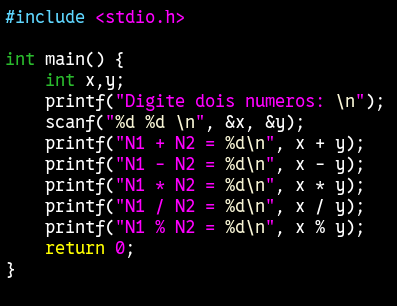
\includegraphics[width=0.3\textwidth]{res/image6.png}
\subsection*{Exercício 2.17}
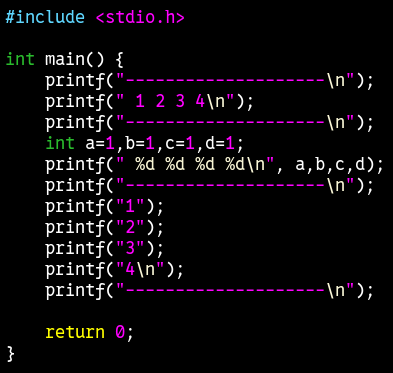
\includegraphics[width=0.3\textwidth]{res/image7.png}
\subsection*{Exercício 2.18}
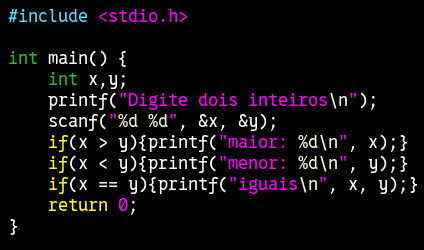
\includegraphics[width=0.3\textwidth]{res/image8.png}
\subsection*{Exercício 2.19}
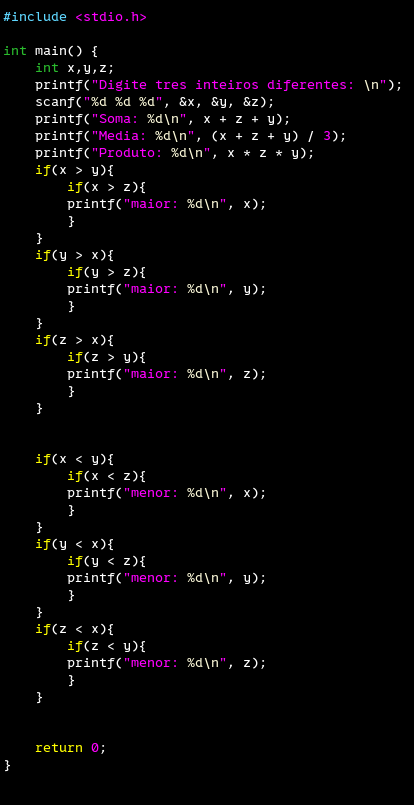
\includegraphics[width=0.3\textwidth]{res/image9.png}
\subsection*{Exercício 2.20}
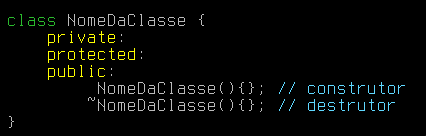
\includegraphics[width=0.3\textwidth]{res/image10.png}
\subsection*{Exercício 2.21}
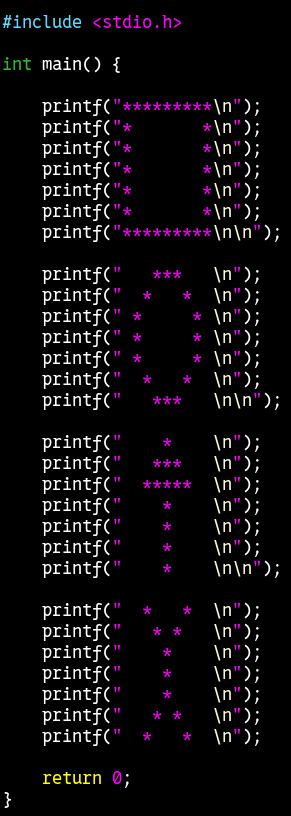
\includegraphics[width=0.3\textwidth]{res/image11.png}
\subsection*{Exercício 2.22}
metade de um triangulo\\ 
\subsection*{Exercício 2.23}
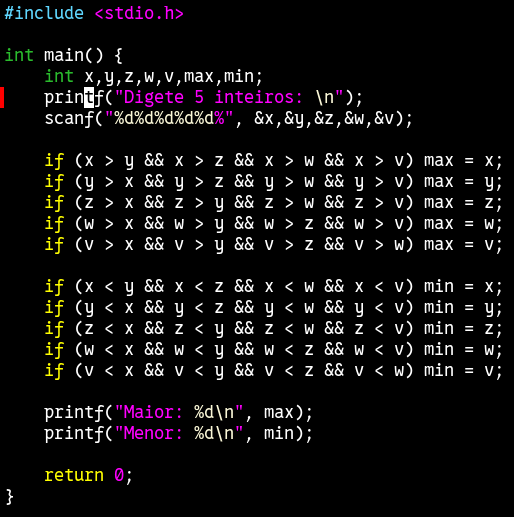
\includegraphics[width=0.3\textwidth]{res/image12.png}
\subsection*{Exercício 2.24}
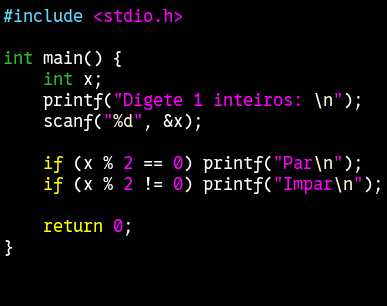
\includegraphics[width=0.3\textwidth]{res/image13.png}
\subsection*{Exercício 2.25}
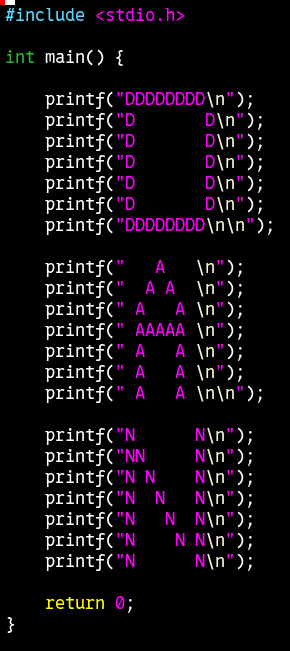
\includegraphics[width=0.3\textwidth]{res/image14.png}
\subsection*{Exercício 2.26}
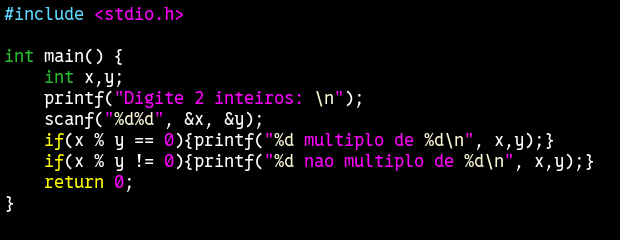
\includegraphics[width=0.3\textwidth]{res/image15.png}
\subsection*{Exercício 2.27}
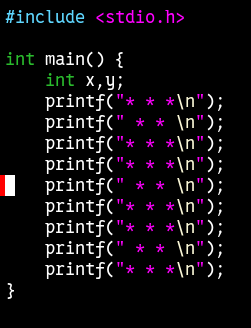
\includegraphics[width=0.3\textwidth]{res/image16.png}
\subsection*{Exercício 2.28}
void,null\\ 
\subsection*{Exercício 2.29}
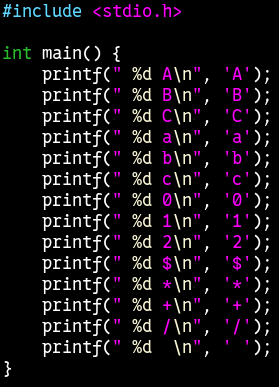
\includegraphics[width=0.3\textwidth]{res/image17.png}
\subsection*{Exercício 2.30}
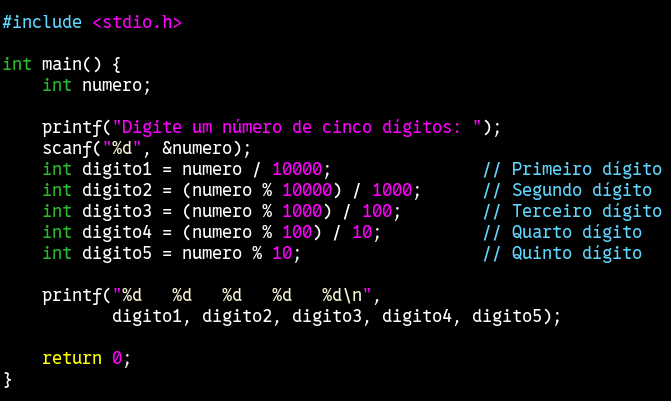
\includegraphics[width=0.3\textwidth]{res/image18.png}
\subsection*{Exercício 2.31}
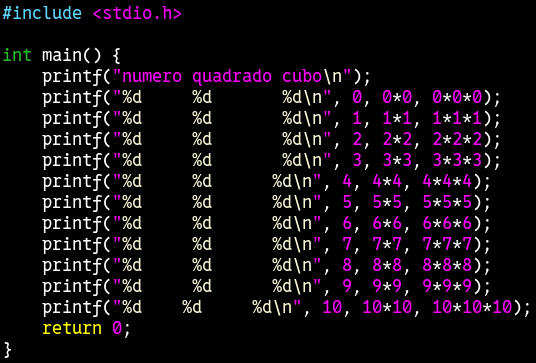
\includegraphics[width=0.3\textwidth]{res/image19.png}
\subsection*{Exercício 2.32}
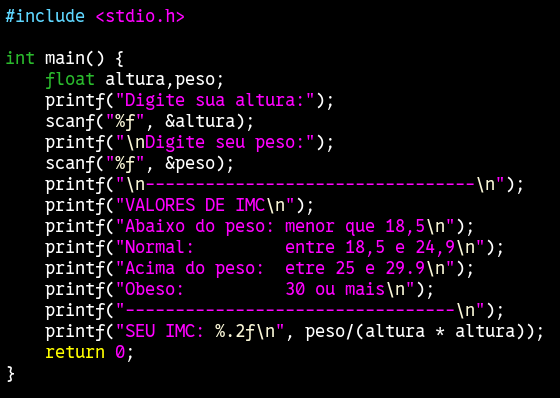
\includegraphics[width=0.3\textwidth]{res/image20.png}
\subsection*{Exercício 2.33}
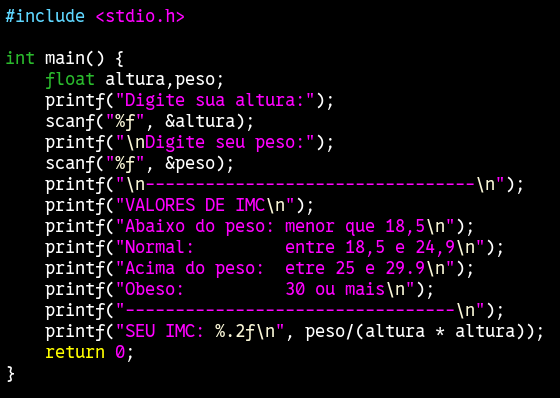
\includegraphics[width=0.3\textwidth]{res/image20.png}
\subsection*{Exercício 3.1}
\begin{enumerate}
    \item[a)] \texttt{algoritmo}
    \item[b)] \texttt{controle de programa}
    \item[c)] \texttt{condicionais}
    \item[d)] \texttt{if, else if, else}
    \item[e)] \texttt{condicionais}
    \item[f)] \texttt{while}
    \item[g)] \texttt{for}
    \item[h)] \texttt{break}
\end{enumerate}
\subsection*{Exercício 3.2}
\begin{enumerate}
    \item[] \texttt{ x += 1 }
    \item[] \texttt{ x++ }
    \item[] \texttt{++x}
    \item[] \texttt{ x = x + 1 }
\end{enumerate}
\subsection*{Exercício 3.3}
\begin{enumerate}
    \item[a] \texttt{ a = x + y + z + x;  }
    \item[b] \texttt{ produto *= 2; }
    \item[c] \texttt{ produto = 2 * produto; }
    \item[d] \texttt{ if(contador > 10){printf("Contador e maoir que 10.")}}
    \item[e] \texttt{--x; x - total }
    \item[f] \texttt{x + total; --x; }
    \item[g] \texttt{......}
    \item[h] \texttt{printf("\%.2f",123.4567);}
    \item[i] \texttt{printf("\%.3f",3.1415);}
\end{enumerate}
\subsection*{Exercício 3.4 pag.103}















\section*{}
\begin{center}
\Huge \textbf{Flash-Card Session}
\end{center}
\vspace{1em} % Espaço vertical
\noindent
Nesta seção, denominada \textbf{Flash-Card Session}, serão armazenados e organizados todos os flash cards criados ao longo do estudo do livro. Cada flash card contém perguntas e respostas que ajudam a revisar e fixar os conceitos importantes abordados no material. 
O objetivo desta seção é fornecer uma forma prática de \textit{recall} ativo, permitindo que o leitor revise rapidamente os pontos principais do livro, reforçando o aprendizado de forma eficiente e contínua.
Recomendo este aplicativo para flash cards \textcolor{blue}{\textbf{\href{https://apps.ankiweb.net/}{https://apps.ankiweb.net/}}} 



\begin{center}
    \colorbox{blue!30}{\Large\textbf{CAPÍTULO 1 ATE 14 EM C}}
\end{center}

\section*{Flash-Card 1 - C Como programar}
O que é  GCC\dotfill Compilador do projeto GNU, compila C, C++, Assembly\\
O que significa GCC\dotfill GNU Compiler Collection\\
O que é  CC\dotfill symlink para o compilador\\
Comentário em bloco em C\dotfill /* */  \\
Comentários são ignorados pelo compilador\dotfill sim\\
Comentário em linha em C\dotfill //\\
Qual o nome desse caracter \textbackslash\, no C\dotfill caractere de escape\\
Como ter o caractere \textbackslash\ em uma string no C\dotfill printf("\textbackslash\textbackslash")\\
C é sensível a maiúscula e minúscula \dotfill sim\\
O que são identificadores no C \dotfill nomes de algo no código\\
Qual o tamanho de um identificador no C \dotfill ilimitado\\
A primeira letra de um identificador de uma variável deve ser\dotfill minúscula\\
O operador de módulo só pode ser usado com\dotfill inteiros\\
Posso fazer isso no C  float \% float \dotfill Não, \% só aceita inteiros\\

\section*{Flash-Card 2 - C Como programar}
Caracteres em C podem ser representados como \dotfill inteiros\\
C tem operador de potência \verb|**| \dotfill não\\
Operador ternário em C \dotfill \verb|? :|\\
C tem quantos operadores ternários? \dotfill 1\\
Esta expressão tem quantos operandos? \verb|a ? b : c| \dotfill 3 operandos\\
Os três únicos \textit{loops} em C \dotfill \verb|for|, \verb|while|, \verb|do..while|\\

\section*{Flash-Card 3 - C Como programar} 
No loop while com uma linha precisa de\{\}\dotfill não\\ 
Qual o nome desse tipo de número no C 1.23\dotfill números de ponto flutuante\\ 
Qual o corpo do operador de cast\dotfill (tipo) expressão\\ 
Cast entre tipos escalares\dotfill converte o valor\\ 
Cast entre ponteiros\dotfill só muda a interpretação dos bits\\ 
O que é operador unário\dotfill operador que aceita somente um operando\\ 
Como imprimir N casas decimais\dotfill \%.nf - \%.2f\\ 
Por padrão qual o tamanho do \%f\dotfill \%.6f\\ 
O C tem quantos operadores de atribuição\dotfill 11\\ 
%Cite todos os operadores de atribuição do C\dotfill \includegraphics[width=0.2\textwidth]{res/image21.png}\\

\section*{Flash-Card 4 - C Como Programar} 
Qual o valor do EOF\dotfill normalmente -1\\ 
O que é um sentinela no C\dotfill valor especial para controlar um laço\\
Quem é o sentinela:\;if(x = 1)\;\{break;\}\dotfill valor sentinela 1\\ 
O loop também pode ser chamado de\dotfill laço\\ 
No C, caracteres podem ser armazenados em\dotfill tipos de dados inteiros\\ 
O que significa EOF\dotfill End Of File (fim do arquivo)\\ 
EOF é de qual biblioteca\dotfill <stdio.h>\\ 
Qual o nome disso \%c \%d\dotfill especificadores de conversão\\ 
Qual a forma de me proteger disso x == 1 (x = 1)\dotfill inverte ( 1 == x )\\ 

\section*{Flash-Card 5 - C Como Programar} 
Qual a melhor forma de manter um programas grandes\dotfill Quebra o projeto grande em varios menores\\ 
Defina o especificador de convencao\dotfill\%f - \%(tipo)\\ 
variaveis de uma funcao sao local ou global\dotfill local\\ 
Definicao de uma funcao\dotfill (tipo-de-retorno) (nome-da-funcao)(parametros){definicoes/instrucoes}\\ 
Qual o nome disso \%f\%d\%s\%lf\dotfill especificadores de formato\\ 
O que e LIFO \dotfill last-in, first-out (LIFO)\\ 
Qual e o conceito do LIFO\dotfill ultimo a entrar primeiro a sair\\ 

\section*{Flash-Card 6 - C Como Programar} 
Cite classes de armazenamento no C\dotfill auto, register, extern, static\\ 
isso e a mesma coisa que int x = 1\dotfill auto int x = 1\\ 
o que e um identificador\dotfill nomes genericos\\ 
Classes de armazenamento definem\dotfill tempo de vida, escopo e visibilidade de uma variavel\\ 
O que e uma funcao recursiva\dotfill funcao que chama a si mesma direta ou indiretamente\\
recursao com funcoes melhora o desempenho\dotfill nao\\ 

\section*{Flash-Card 7 - C Como Programar} 
Qual nome desses números x C[x]\dotfill índice\\ 
O que isso faz int n[10] = \{0\}; \dotfill Inicializa todos os elementos com zero\\ 
int C[\;]\dotfill o tamanho do array será o tamanho da lista de inicializadores\\
Qual nome, \#define\dotfill diretiva do pré-processador\\ 
O que são protótipos de função\dotfill funções declaradas sem corpo\\ 
Especificador de conversão para endereços\dotfill \%p\\ 
int x[2][2] =\dotfill \{\{1,1\},\{1,1\}\}\\ 
Variáveis de ponteiro recebem\dotfill endereços de memória\\  
Um ponteiro pode ser inicializado com\dotfill NULL, 0\\ 
Único valor inteiro para atribuir a um ponteiro\dotfill 0\\ 
\&\dotfill operador de endereço\\  
O que o operador \& faz\dotfill retorna o endereço do seu operando\\
Defina \&, entre operador unário ou ternário\dotfill operador unário\\ 
int *p\dotfill declara um ponteiro\\ 
*p\dotfill usa o ponteiro para acessar o valor\\ 
Cite os operadores de ponteiros\dotfill *, \&, \%p\\ 

\section*{Flash-Card 8 - C Como Programar} 
Qual o ultimo caracter em uma string no C\dotfill caractere nulo \textbackslash0\\ 
Uma string tambem pode ser considerada um\dotfill ponteiro\\ 
Lib para tratamento de caracteres\dotfill ctype.h\\ 
Qual tipo de dado o ctype.h trabalha\dotfill char\\ 
Lib para tratamento de String\dotfill string.h\\ 
\%s, o que ele faz no printf\dotfill imprime ate o caractere nulo\\ 
Strings em C terminam com\dotfill \textbackslash0\\ 
Qual o nome disso \textbackslash0\dotfill caractere nulo\\ 
Qual especificador de formato eu uso para char\dotfill \%c\\  
Struct pode ser chamado de \dotfill estruturas, agregacoes\\ 
Dois operadores sao usados para acessar estruturas\dotfill (->)(.)\\ 
struct, quando usar (->)\dotfill acessa por ponteiro\\ 
struct, quando usar (.)\dotfill acesso normal\\ 
Qual o nome desse operador (.)\dotfill operador de membro de estrutura\\ 
Qual o nome desse operador (->)\dotfill operador de ponteiro de estrutura\\ 

\section*{Flash-Card 9 - C Como Programar} 
O que é FILE em C\dotfill estrutura para manipular arquivos\\ 
Onde a estrutura FILE é definida\dotfill stdio.h\\ 
Quais são os canais de comunicação de um sistema\dotfill stdin, stdout, stderr\\ 
Listas encadeadas são feitas com\dotfill estrutura auto-referenciada\\ 
Todas as diretivas do pré-processador começam com\dotfill \#\\ 
O que vem antes da compilação no C\dotfill pré-processamento\\ 
Duas formas de diretivas de \#include\dotfill \#include <> ou ''''\\ 
Quando usar \#include <>\dotfill bibliotecas padrão\\ 
Quando usar \#include ''''\dotfill bibliotecas não padrão\\ 
Corpo do \#define\dotfill \#define identificador texto-substituto\\ 
O que o \#define faz\dotfill substitui o texto por outro\\ 
Algumas outras macros\dotfill \#error, \#pragma, \#line\\ 
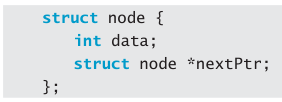
\includegraphics[width=0.3\textwidth]{res/image26.png}\dotfill estrutura auto-referenciada\\   
Defina construtores de tipo em C\dotfill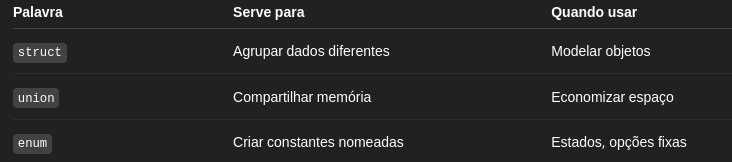
\includegraphics[width=0.5\textwidth]{res/image25.png}\\ 
Operadores sobre bits no C\dotfill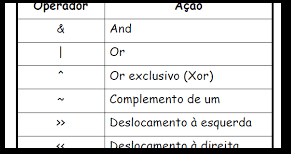
\includegraphics[width=0.2\textwidth]{res/image23.png}\\ 
Operadores de atribuição sobre bits no C\dotfill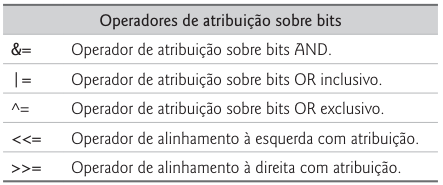
\includegraphics[width=0.3\textwidth]{res/image24.png}\\ 

\begin{center}
    \colorbox{blue!30}{\Large\textbf{CAPÍTULO 15 ATE 24 EM C++}}
\end{center}

\section*{Flash-Card 11 - C Como Programar} 
Nomes de extensões de arquivos C++\dotfill .cpp, .cxx, .C (maiúsculo)\\ 
Comentário de linha e de bloco no C++\dotfill //, /* */\\ 
Qual o compilador do C++\dotfill g++\\ 
Qual a principal biblioteca de entrada e saída do C++\dotfill iostream\\ 
Variáveis por referência criam cópias em funções\dotfill não\\ 
Defina isso \texttt{void soma(int \&x)}\dotfill passagem por referência\\
Como se lê \texttt{int \&x}\dotfill x é uma referência para a variável original\\
\texttt{using} \dotfill adiciona um único método de um namespace\\
\texttt{using namespace} \dotfill adiciona todo o namespace (biblioteca)\\

\section*{Flash-Card 12 - C Como Programar} 
Sobrecarga de função em soma(int x, int x)\dotfill \_\_z4somaii\\
Mesma função, código, mas entrada diferente\dotfill template de função\\ 
O destrutor precisa ter o mesmo nome da classe no C++\dotfill sim\\ 
Class Pessoa{}, como fica o destrutor\dotfill \textasciitilde Pessoa(){}\\ 
C++ tem palavras reservadas para métodos get, set\dotfill não\\ 
Defina uma classe em C++\dotfill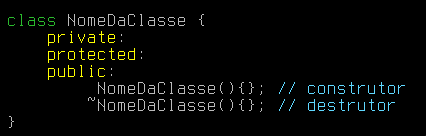
\includegraphics[width=0.5\textwidth]{res/image10.png}\\

\section*{Flash-Card 13 - C Como Programar} 
Um construtor, pode retorna valores no C++\dotfill nao\\ 
Qual o nome disso no C++,"::"\dotfill operador binario de resolucao de escopo\\ 
%-------507



\section*{Notas apra pesquisa}
x++ ou ++x, 1++ ou ++1\\   
repeticao definida\\ 
repeticao indefinida\\ 
estudar aaa estrutgura de switch\\ 
oque significa ascii\\ 
getcahr();\\ 
O que acontece se eu deixar assim scanf("\%d \%d \%d ", \&x, \&y, \&z);\dotfill bloqueia o scanf()\\ 
computacao conversacional\\  
computacao interativa ou reativa\\ 
programacao estruturada\\ 
programacao procedural\\  
oque significa ANSI\\  
oque significa ISO\\ 
livro pj.Plauger,The standard C library\\ 
Decomposisao de funcoes \\ 
todos os especificadores de formato\\ 
oque ee LIFO\\ 
stack ouverflow - estouro de pilha\\ 
estude numeros aleatorios em C..\\ 
algoritmo de numeros aleatorios\\ 
como passar um array para um funcao\\ 
algoritmo bubble sort ee sinking sort\\ 
aritmetic de ponteiros\\ 
estude const com ponteiros\\ 
apreda aaa usar o sizeof\\ 
C, strutura autorreferenciada\\ 
diferenca entre struct, typedef struct\\ 
constantes simbolicas\\ 
esatudar abrir fechar arquivos\\ 
abrir fechar arquivos \\ 
estudar o goto no C\\ 
*(bptr + 3)\\ 
 *x = *x\\ 














\end{document}
Comentario em bloco em C\dotfill /* */  \\
